\documentclass[12pt,a4paper]{article}

\usepackage[a4paper,top=20mm,bottom=22mm,left=25mm,right=20mm]{geometry}
\usepackage{fontspec}
\usepackage{xcolor}
\usepackage{graphicx}
\usepackage{hyperref}
\usepackage{fancyhdr}
\usepackage{titlesec}
\usepackage{enumitem}
\usepackage{booktabs}
\usepackage{longtable}
\usepackage{array}
\usepackage{colortbl}
\usepackage{listings}
\usepackage{caption}
\usepackage{float}
\usepackage{tikz}
\usetikzlibrary{arrows.meta,positioning}
\usepackage{tocloft}
\usepackage{etoolbox}
\usepackage{needspace}

\setmainfont{Times New Roman}
\setmonofont{Menlo}
\graphicspath{{../report_src/img/}}

\definecolor{linkblue}{HTML}{1D3F7A}
\definecolor{passgreen}{HTML}{0A6B2D}
\definecolor{headbg}{HTML}{E9EDF3}
\definecolor{codebg}{HTML}{F4F6F9}
\definecolor{coderule}{HTML}{D6DBE3}
\definecolor{footgray}{HTML}{444444}

\linespread{1.2}
\setlength{\parindent}{0pt}
\setlength{\parskip}{6pt plus 1pt}
\setlength{\emergencystretch}{8em}
\tolerance=4000

\hypersetup{
  hidelinks,
  unicode=true,
  pdftitle={V-1-4_BD1_Report -- Kernel Data Structures},
  pdfauthor={V-1-4 team}
}

\pagestyle{fancy}
\fancyhf{}
\fancyfoot[C]{\fontsize{9}{11}\selectfont\color{footgray}\thepage}
\renewcommand{\headrulewidth}{0pt}
\renewcommand{\footrulewidth}{0pt}

\titleformat{\section}{\normalfont\fontsize{15}{18}\selectfont\bfseries}{}{0pt}{}
\titlespacing*{\section}{0pt}{16pt}{6pt}
\titleformat{\subsection}{\normalfont\fontsize{13.5}{16}\selectfont\bfseries}{}{0pt}{}
\titlespacing*{\subsection}{0pt}{14pt}{5pt}
\titleformat{\subsubsection}{\normalfont\fontsize{12.5}{15}\selectfont\bfseries}{}{0pt}{}
\titlespacing*{\subsubsection}{0pt}{12pt}{4pt}

\newcommand{\hthree}[1]{%
  \par\Needspace{4\baselineskip}\addvspace{10pt}%
  {\fontsize{12.5}{15}\selectfont\bfseries #1\par}%
  \addvspace{3pt}%
}

\newcommand{\manualsection}[1]{%
  \par\Needspace{5\baselineskip}\addvspace{18pt}%
  {\fontsize{16}{19}\selectfont\bfseries\color{linkblue} #1\par}%
  \addvspace{6pt}%
}
\newcommand{\manualsubsection}[1]{%
  \par\Needspace{4\baselineskip}\addvspace{14pt}%
  {\fontsize{13}{16}\selectfont\bfseries #1\par}%
  \addvspace{4pt}%
}

\newcommand{\code}[1]{{\fontsize{10}{12}\selectfont\texttt{\detokenize{#1}}}}

\captionsetup{font={small,it}, justification=centering, skip=3pt, labelformat=empty}

\lstdefinestyle{kds}{
  basicstyle=\ttfamily\fontsize{8.5}{10.5}\selectfont,
  columns=fixed,
  basewidth=0.602em,
  keepspaces=true,
  breaklines=true,
  breakatwhitespace=false,
  showstringspaces=false,
  frame=single,
  framerule=0.4pt,
  rulecolor=\color{coderule},
  backgroundcolor=\color{codebg},
  xleftmargin=0pt,
  xrightmargin=0pt,
  aboveskip=4pt,
  belowskip=8pt,
  extendedchars=true,
  inputencoding=utf8
}
\lstnewenvironment{codeblock}{\lstset{style=kds}}{}

\newcolumntype{L}[1]{>{\raggedright\arraybackslash}p{#1}}
\AtBeginEnvironment{longtable}{\fontsize{10.5}{13}\selectfont}
\renewcommand{\arraystretch}{1.15}
\setlength{\tabcolsep}{4pt}

\renewcommand{\contentsname}{Агуулга}
\renewcommand{\cfttoctitlefont}{\fontsize{15}{18}\selectfont\bfseries}
\setlength{\cftbeforetoctitleskip}{0pt}
\setlength{\cftaftertoctitleskip}{12pt}
\renewcommand{\cftsecleader}{\cftdotfill{\cftdotsep}}
\setlength{\cftsecindent}{0pt}
\setlength{\cftsecnumwidth}{0pt}
\renewcommand{\cftsecfont}{\normalfont}
\renewcommand{\cftsecpagefont}{\normalfont}
\setlength{\cftbeforesecskip}{4pt}
\setlength{\cftsecnumwidth}{0pt}

\setlength{\LTpre}{4pt}
\setlength{\LTpost}{8pt}

\AddToHook{cmd/section/before}{\Needspace{4\baselineskip}}


\begin{document}

% ---------------------------------------------------------------------------
% Нүүр хуудас
% ---------------------------------------------------------------------------
\begin{titlepage}
\thispagestyle{empty}
\centering
{\fontsize{14}{19}\selectfont\bfseries
ШИНЖЛЭХ УХААН ТЕХНОЛОГИЙН ИХ СУРГУУЛЬ\\[2pt]
МЭДЭЭЛЭЛ, ХОЛБООНЫ ТЕХНОЛОГИЙН СУРГУУЛЬ\par}

\vspace{10mm}

\includegraphics[width=30mm]{logo.png}
\vspace{9mm}

{\fontsize{13}{16}\selectfont F.CSM302 Үйлдлийн систем · Бие даалт 1\par}
\vspace{3mm}
{\fontsize{24}{29}\selectfont\bfseries Судалгаа, хэрэгжилт, туршилтын тайлан\par}
\vspace{2mm}
{\fontsize{17}{21}\selectfont\bfseries Kernel Data Structures\par}
\vspace{5mm}

{\fontsize{13}{16}\selectfont
Хуваарилалтын код: \textbf{V-1-4} · Үзүүлэлт: Kernel structure graph · Бүлэг 3 -- Processes\par}
\vspace{1mm}
{\fontsize{13}{16}\selectfont
Сурах бичиг: Chapter 1 Introduction, 1.9 Kernel Data Structures (p. 36)\par}
\vspace{1mm}
{\fontsize{13}{16}\selectfont
GitHub: github.com/grl059/OS\_BD1\par}

\vspace{12mm}
{\fontsize{12.5}{15}\selectfont
\begin{tabular}{@{}ll@{}}
Хичээл заасан багш: & Г. Ганбат (F.CS10)\\
Гүйцэтгэсэн баг: & Н. Ням-Од (B222270805)\\
 & А. Гэрэл (B241940001)\\
 & А. Номин (B242270088)\\
 & Э. Мягмаршагай (B241910001)\\
 & О. Хүслэн (B241910020)\\
 & Ч. Түмэншагай (B160910830)\\
\end{tabular}\par}

\vfill
{\fontsize{12.5}{15}\selectfont
2026--2027 оны хичээлийн жилийн намар · Семинарын цаг: 5-1 пар\\
Улаанбаатар\par}
\end{titlepage}
\setcounter{page}{2}

% ---------------------------------------------------------------------------
% Агуулга
% ---------------------------------------------------------------------------
\tableofcontents
\thispagestyle{fancy}
\clearpage

% ---------------------------------------------------------------------------
% Хураангуй
% ---------------------------------------------------------------------------
\section*{Хураангуй}
\phantomsection\addcontentsline{toc}{section}{Хураангуй}
\noindent\rule{\textwidth}{1.2pt}\par\vspace{6pt}

\textbf{Асуудал.} Kernel процесс, нөөц, файлуудаа холбоост жагсаалт, дараалал, стек, bitmap, хэш хүснэгт, мод зэрэг өгөгдлийн бүтцээр удирддаг. Эдгээрт элемент нэмэх, устгах, хайх үед бүтэц хэрхэн өөрчлөгддөгийг нүдээр харуулж, хэрэгжилтийг нь нотлох шаардлагатай.

\textbf{Шийдэл.} Linux-ийн \code{list_head}-ийн next/prev семантикийг C-ээр дахин бичиж, долоон бүтэц (жагсаалт, queue, stack, bitmap, hash map, BST/AVL мод, PCB бүхий ready queue ба FCFS/Round Robin scheduler) бүхий командын интерпретатор (\code{kds}) бүтээв. Энэ C программд \code{--json} горим нэмж, команд бүрийн дараах бүтцийн төлөвийг JSON хэлбэрээр гаргадаг болгов. Веб дээр ажилладаг хэрэглэгчийн интерфэйс (Next.js, \code{web/} хавтас) нь тэр JSON-ыг C программаас шууд авч, өөрөө юу ч тооцоолохгүйгээр зурж харуулдаг -- өөрөөр хэлбэл, нэг л «бодол» (логик) байдаг: C. Веб нь түүнийг зөвхөн дэлгэцэнд үзүүлнэ. Сурах бичгийн 3-р бүлгийн Programming Project-ийн дагуу kernel module нь \code{struct color} жагсаалт болон \code{start} параметртэй Collatz дарааллын жагсаалтыг kernel орчинд үүсгэж, устгана.

\textbf{Туршилт.} 8 жишээ скрипт ба 5000×8 командын stress тест ASan/UBSan-тай давсан (GitHub Actions-ийн Linux job; macOS 26 дээр ASan runtime эхлэхэд чиддэг асуудлаар \code{make SAN=0} ашигласан). Текст гаралт ба \code{--json} гаралтыг нэг C программаас зэрэг гаргаж, 40\,000 санамсаргүй командад (8 seed × 5000, тэр дотор AVL) мөр мөрөөрөө ижил мессеж өгснийг баталгаажуулсан. AVL-ийн өндрийн хязгаарыг 30 санамсаргүй гүйлтээр шалгасан. GitHub Actions дээр C программ ба веб аппыг автоматаар build, тест хийдэг CI тохируулсан. Kernel module-ийн өмнөх хувилбар Ubuntu 24.04 (kernel 6.11.0-17) дээр insmod/rmmod хийгдсэн.

\textbf{Гол үр дүн.} Оролт, огноо, хязгаарыг шалгадаг, хэрэглэгч өөр өгөгдлөөр дахин туршиж болох, терминал (CLI) ба веб хуудас хоёулаа яг нэг C программаас гарсан мэдээллийг харуулдаг хэрэгсэл бүтээгдсэн.

% ---------------------------------------------------------------------------
% 1. Удиртгал
% ---------------------------------------------------------------------------
\section*{1. Удиртгал}
\phantomsection\addcontentsline{toc}{section}{1. Удиртгал}

Үйлдлийн системийн kernel нь процессын жагсаалт, ready queue, bitmap (нөөц чөлөөтэй эсэх), хэш хүснэгт (хурдан хайлт), модон бүтэц (scheduler, санах ой) зэргийг өгөгдлийн бүтцээр удирддаг. Төслийн \textbf{зорилго} нь эдгээрийн үндсэн үйлдлийг хэрэгжүүлж, үйлдэл бүрийн дараах төлөвийг нүдэнд харагдахуйц болгох явдал юм.

\textbf{Ач холбогдол.} \code{list_head} бол Linux kernel-ийн хамгийн их хэрэглэгддэг бүтэц бөгөөд \code{task_struct} (PCB), ready queue зэрэг нь түүн дээр суурилдаг. Үүнийг ойлгох нь 3-р бүлгийн «Processes» сэдвийн суурь болно.

\textbf{Хамрах хүрээ.} Хэрэглэгчийн орчны загвар (C, CLI), түүн дээр суурилсан веб хуудас (Next.js), мөн нэг kernel module. Бодит Linux scheduler-т холбогдохгүй.

% ---------------------------------------------------------------------------
% 2. Сурах бичгийн шаардлага
% ---------------------------------------------------------------------------
\section*{2. Сурах бичгийн шаардлага}
\phantomsection\addcontentsline{toc}{section}{2. Сурах бичгийн шаардлага}

\textbf{Хуваарилалт:} код 4, «Kernel Data Structures», үзүүлэлт «Kernel structure graph», бүлэг 3 -- Processes. Онолын хэсэг нь \textbf{Chapter 1 Introduction-ийн 1.9 Kernel Data Structures (p. 36)}. \textbf{Хүрэх үр дүн:} «Сурах бичигт заасан kernel data structure-ийн хэрэглээг хэрэгжүүлж, элемент нэмэх, устгах, хайх үйлдлийн дараах бүтцийг графаар харуулна.»

Operating System Concepts-ийн 3-р бүлгийн Programming Project «Kernel Data Structures» нь Chapter 1-ийн 1.9 Kernel Data Structures (p. 36)-д тайлбарласан бүтцүүд дээр тулгуурласан хоёр хэсэгтэй:

\begin{itemize}[leftmargin=20pt,itemsep=2pt,topsep=2pt]
  \item \textbf{Part I:} \code{struct color {red, blue, green; struct list_head list;}} төрлийн элементүүдийг kernel module дотор жагсаалтад нэмж, \code{list_for_each_entry}-ээр гүйлгэн хэвлэх, module-ийг буулгахад \code{list_for_each_entry_safe}-ээр устгаж санах ойг чөлөөлөх.
  \item \textbf{Part II:} module-д \code{start} параметр дамжуулж (\code{module_param}), Collatz дарааллыг (тэгш бол n/2, сондгой бол 3n+1, 1 хүртэл) холбоост жагсаалтад хадгалан хэвлэх, буулгахад устгах.
\end{itemize}

Доорх хүснэгт нь шаардлага бүрийг хэрэгжилт ба баталгаажуулалттай холбосон.

{\fontsize{9.5}{12}\selectfont
\begin{longtable}{|L{0.21\textwidth}|L{0.22\textwidth}|L{0.27\textwidth}|L{0.22\textwidth}|}
\hline
\rowcolor{headbg}\textbf{Шаардлага} & \textbf{Хэрэгжилт} & \textbf{Нэмэх / устгах / хайх} & \textbf{Баталгаа} \\ \hline
\endfirsthead
\hline
\rowcolor{headbg}\textbf{Шаардлага} & \textbf{Хэрэгжилт} & \textbf{Нэмэх / устгах / хайх} & \textbf{Баталгаа} \\ \hline
\endhead
Ch.3 Part I: struct color жагсаалт & \code{kds_module.c}, \code{color_list} & \code{list_add_tail}, \code{list_del}, \code{list_for_each_entry} & \code{run_module_}\allowbreak\code{test.sh}, dmesg \\ \hline
Ch.3 Part II: Collatz, \code{start} параметр & \code{kds_module.c}, \code{module_param}\allowbreak\code{(start)}, 1..1\,000\,000 & \code{list_add_tail}, \code{list_del} & start=25, 15, 0 (татгалзана) \\ \hline
1.9.1 Холбоост жагсаалт (list\_head) & Давхар холбоост дугуй жагсаалт (struct birthday) & add\_head, add\_tail, del, find & textbook, search, веб «Чөлөөт горим» \\ \hline
1.9.1 Stack (LIFO) & list\_head, дээд талаас нэмж авна & push, pop, find & all\_structures, search \\ \hline
1.9.1 Queue (FIFO) & list\_head, төгсгөлд нэмж эхнээс авна & push, pop, find & all\_structures, search \\ \hline
1.9.2 Binary search tree & Энгийн BST (хамгийн муу $O(n)$) & insert, delete, find & search: 1--5 $\rightarrow$ өндөр 5 \\ \hline
1.9.2 Тэнцвэржсэн мод ($O(\lg n)$) & AVL (\code{tree mode avl}) & insert, delete, find & search, avl\_check: 1--7 $\rightarrow$ өндөр 3 \\ \hline
1.9.3 Хэш функц ба hash map & Кодын нийлбэр mod n; collision-д bucket доторх hlist\_head жагсаалт; ачаалал > 0.75 бол bucket $\times$2 (\code{hash auto on}), гараар \code{rehash} & put, del, get, rehash, stats & search, hash\_resize \\ \hline
Нэмэлт: red-black мод (CFS-ийн мод) & \code{rb} горим: өнгө, black-height, эргүүлэлтийн тоо & insert, delete, find & rb\_heap, rb\_check (30 seed) \\ \hline
Нэмэлт: min-heap (priority queue) & массив дээрх овоолго, багтаамж 16, swap тоо & push, pop, peek & rb\_heap, rb\_check (10 seed) \\ \hline
1.9.4 Bitmap & n = 1..128 бит & set, clear, test & all\_structures, errors \\ \hline
«Processes» холбоос & PCB + list\_head ready queue, FCFS, Round Robin & proc new / дуусах / sched print & scheduler, scheduler\_full \\ \hline
\end{longtable}
\par}

\textbf{Харуулах шаардлага:} веб хуудас нь бүтэц бүрийн нэмэх, устгах, хайх үйлдлийн дараах төлөвийг граф хэлбэрээр шууд зурдаг (6-р хэсэг).

% ---------------------------------------------------------------------------
% 3. Онолын үндэс
% ---------------------------------------------------------------------------
\section*{3. Онолын үндэс}
\phantomsection\addcontentsline{toc}{section}{3. Онолын үндэс}

\textbf{Эх сурвалж:} Silberschatz, Galvin, Gagne, \textit{Operating System Concepts}, 10th ed., Chapter 1 Introduction, 1.9 Kernel Data Structures, p. 36 (1.9.1 жагсаалт/stack/queue, 1.9.2 мод, 1.9.3 hash, 1.9.4 bitmap).

\textbf{list\_head} нь intrusive, давхар холбоост, дугуй жагсаалт юм. Node нь өгөгдлийн struct дотор \code{list_head} талбар агуулж, \code{container_of} макро нь талбарын хаягаас эзэн struct-ийг сэргээнэ. Нэмэх, устгах үйлдэл $O(1)$, хайх нь $O(n)$.

\textbf{Queue (FIFO)} нь tail-д нэмж head-ээс авдаг. Kernel-ийн ready queue ийм зарчмаар ажилладаг. \textbf{Stack (LIFO)} нь head-д нэмж head-ээс авдаг.

\textbf{Bitmap}-д 1 бит нь 1 нөөцийг илэрхийлнэ. set/clear/test нь $O(1)$ бөгөөд Boolean массиваас 8 дахин бага зай эзэлнэ.

\textbf{Binary search tree}-д зүүн $<$ үндэс $<$ баруун байна. Дундаж хайлт $O(\lg n)$, харин эрэмбэлсэн оролтод мод нэг шугам болж хамгийн муу тохиолдол $O(n)$ болно. Тэнцвэржсэн мод n элементэд ойролцоогоор $\lg n$ түвшинтэй байдаг. Linux red-black мод ашигладаг бол бид ижил зорилготой AVL модоор (өндрийн зөрүү $\le 1$, эргүүлэлт) загварчилсан.

\textbf{Hash map}-д хэш функц түлхүүрийг хүснэгтийн индекс болгож, ихэнх тохиолдолд $O(1)$ хайлт өгнө. Хоёр түлхүүр нэг индекст таарвал (collision) тухайн bucket-д жагсаалт залгана. Collision олшрох тусам хайлт $O(n)$ руу ойртоно.

\textbf{Процесс ба scheduler.} Процесс бүр PCB-тэй байдаг (Linux-д \code{task_struct}). Бэлэн процессууд ready queue-д зогсоно. FCFS нь процессыг дуустал нь ажиллуулна. Round Robin нь процесс бүрд квант хугацаа өгч, дуусаагүй бол дарааллын төгсгөлд буцаана. Хүлээлтийн хугацааг нийт үргэлжилсэн хугацаанаас ажлын хугацааг хасаж олно.

\textbf{Kernel module ба параметр.} \code{module_param(name, type, perm)} нь \code{insmod kds_module.ko start=15} хэлбэрээр утга дамжуулах боломж олгоно. Init амжилтгүй болбол \code{module_exit} дуудагдахгүй тул init өөрөө нөөцөө чөлөөлөх ёстой. Нийтлэг алдаанууд: \code{list_del}-ийн дараа pointer ашиглах, node чөлөөлөхгүй үлдээх (leak), гүйлгэж байхдаа устгах (энэ үед \code{_safe} хувилбар хэрэгтэй).

% ---------------------------------------------------------------------------
% 4. Системийн зохиомж
% ---------------------------------------------------------------------------
\section*{4. Системийн зохиомж}
\phantomsection\addcontentsline{toc}{section}{4. Системийн зохиомж}

\textbf{Компонентууд:}

\begin{itemize}[leftmargin=20pt,itemsep=2pt,topsep=2pt]
  \item \textbf{(a) src/user/kds.c} -- командын интерпретатор ба 9 бүтэц (жагсаалт, queue, stack, bitmap, hash, BST/AVL мод, red-black мод, min-heap, процесс/хуваарилагч). Жагсаалт, queue, stack, hash-ийн bucket, ready queue бүгд нэг \code{list_head} хэрэгжилтийг ашиглана. Энэ файл дотор ердийн текст мессеж гаргадаг горимоос гадна \code{--json} горим бий: команд тус бүрийн дараа бүтцийн бүх төлөвийг нэг JSON мөр болгож бичдэг.
  \item \textbf{(b) web/} -- Next.js (React, TypeScript) дээр бичигдсэн веб апп. Хэрэглэгч товч дарах эсвэл команд бичих үед веб апп сервер талд \code{kds --json}-ыг ажиллуулж, буцаж ирсэн JSON мөр бүрийг дэлгэц дээр граф болгож зурна. Веб апп өөрөө ямар ч бүтцийн логик (нэмэх, устгах, хайх дүрэм) агуулдаггүй -- зөвхөн C программаас ирсэн төлөвийг дүрсэлж харуулна. Нүүр (7 шатны жагсаалт ба дээд цэс), «Чөлөөт горим» (бүтэц сонгож, үйлдлийн товчоор турших), «Хичээл» (7 шат: алхам бүрт Багшийн тайлбар ба монгол дуу, асуулттай тест), «Тухай» хуудастай.
  \item \textbf{(c) \texttt{src/kernel/kds\_module.c}} -- kernel орчинд ажиллах хувилбар: color, Collatz, birthday жагсаалт, kfifo, bitmap, мөн \code{hashtable.h}, \code{rbtree.h} болон \code{/proc/kds}.
  \item \textbf{(d) tests/} -- C-ийн текст гаралт ба \code{--json} гаралтыг хооронд нь, мөн хүлээгдэх гаралттай харьцуулдаг тестүүд.
\end{itemize}

\textbf{Өгөгдлийн урсгал:} хэрэглэгчийн команд (товч, командын мөр эсвэл script) $\rightarrow$ веб апп серверийн тал нь командыг \code{kds --json}-д дамжуулна $\rightarrow$ C программ бүтцийн төлөвийг шинэчилж, нэг JSON мөр болгож буцаана $\rightarrow$ веб апп тэр JSON-оос шууд график зурна. Тооцоолол бүгд C дотор хийгддэг тул веб дээр харагдах зураг бодит ажиллагаанаас хэзээ ч зөрөхгүй.

\begin{figure}[H]
\centering
\begin{tikzpicture}[
  box/.style={draw, rounded corners=1pt, align=center,
              font=\ttfamily\fontsize{8.5}{10.5}\selectfont,
              inner sep=4pt, minimum height=11mm},
  arr/.style={-{Latex[length=2mm]}, thick}
]
\node[font=\ttfamily\fontsize{8.5}{10.5}\selectfont, align=center] (input)
  {товч / команд / examples/*.txt\\(веб хуудас дээр)};
\node[box, below=8mm of input] (kds) {kds --json\\(интерпретатор)};
\node[box, right=24mm of kds, text width=52mm] (web)
  {веб апп: graph/log\\(Next.js, зөвхөн дүрслэл)};
\draw[arr] (input) -- (kds);
\draw[arr] (kds) -- node[above, font=\ttfamily\fontsize{8}{10}\selectfont]{JSON (state)} (web);
\end{tikzpicture}
\caption*{Өгөгдлийн урсгал: команд C программ руу, төлөв JSON хэлбэрээр веб рүү.}
\end{figure}

% ---------------------------------------------------------------------------
% 5. Хэрэгжилт
% ---------------------------------------------------------------------------
\section*{5. Хэрэгжилт}
\phantomsection\addcontentsline{toc}{section}{5. Хэрэгжилт}

\textbf{Хэл ба хэрэгсэл:} C (gcc, \code{-Wall -Wextra -fsanitize=address,undefined}), JavaScript (HTML/SVG, сан ашиглаагүй), kernel C (Kbuild), туршилтад Python 3 ба Node.js.

\textbf{Гол шийдлүүд:}

\begin{enumerate}[leftmargin=22pt,itemsep=2pt,topsep=2pt]
  \item \code{list.h}-ийн \code{__list_add}, \code{list_add}, \code{list_add_tail}, \code{list_del}, \code{list_for_each(_safe)}, \code{container_of}-ийг өөрсдөө бичсэн.
  \item Queue ба stack нь ижил list\_head-ийг хуваалцах бөгөөд зөвхөн нэмэх талаараа ялгарна. Багтаамж нь 8.
  \item Огноо шалгахдаа өндөр жилийг тооцно: 4-т хуваагддаг ба 100-д хуваагддаггүй, эсвэл 400-д хуваагддаг.
  \item Модноос хоёр хүүтэй node устгахдаа баруун дэд модны хамгийн бага утгаар орлуулна. AVL горимд буцах замдаа \code{bal()} нь rotl/rotr эргүүлэлтээр тэнцвэржүүлнэ. Модны төрлийг зөвхөн хоосон үед солино.
  \item Hash map нь 1--16 bucket-тэй. Хэш функц нь тэмдэгтүүдийн кодын нийлбэр mod n. Collision-ийг bucket доторх list\_head жагсаалтаар шийднэ (chaining). Нийт 24 элементээр хязгаарласан. \code{get} үйлдэл хайлтын алхмын тоог мэдээлнэ.
  \item PCB нь \code{struct pcb {pid, name, rem, slice, list_head}} бүтэцтэй. Ready queue-д \code{list_add_tail}-аар нэмж, эхний элементийг \code{list_del}-ээр авч CPU-д өгнө. \code{sched tick} бүрд CPU 1 тик ажиллана. FCFS нь процессыг дуустал ажиллуулна. RR-д квант дуусвал процесс дарааллын төгсгөлд буцна (preempt). Амьд процессын тоо 8 хүртэл.
  \item Хайх үйлдэл бүх бүтцэд байна: list find (индекс), queue/stack find (байрлал), tree find, bitmap test, hash get.
  \item \textbf{Kernel module:} init дотор color (4 элемент), Collatz (start-аас 1 хүртэл, хамгаалалтын хязгаар 1000 гишүүн), birthday, kfifo, bitmap-ийг үүсгэнэ. \code{start} нь 1..1\,000\,000 мужаас гадуур бол \code{-EINVAL} буцааж module ачаалагдахгүй. \code{kmalloc} алдаа гарвал \code{goto fail}-аар бүх жагсаалтыг цэвэрлэнэ. Exit дотор \code{list_for_each_entry_safe}-ээр элемент бүрийг хэвлэж устгана.
  \item Веб апп нь C программыг дахин бичсэн хуулбар биш. Нэг л дүрэм, нэг л код (\code{kds.c}) байдаг бөгөөд веб зөвхөн түүний \code{--json} гаралтыг уншиж зурдаг. Иймээс «веб ба C-ийн гаралт зөрөх» эрсдэл угаасаа байхгүй -- тэд угаасаа нэг эх сурвалжтай.
\end{enumerate}

\hthree{5.1 GitHub дээрх ажиллагаа}

Repository: \code{github.com/grl059/OS_BD1} (салбар \code{main}). Бүтэц нь удирдамжийн 6-р хэсгийн дагуу: \code{README.md} (нэр, код, зорилго, Quick Start, AI тэмдэглэл), \code{src/}, \code{tests/}, \code{examples/}, \code{docs/} (Manual, Report, screenshot, тайлангийн эх HTML). Build-ийн гаралт болон гарын үсгийн түлхүүрийг \code{.gitignore}-оор хассан. 9-р долоо хоногт нийтэлсэн хувилбар нь \code{v1.0.0} tag ба GitHub Release.

{\fontsize{9.5}{12}\selectfont
\begin{longtable}{|L{0.17\textwidth}|L{0.26\textwidth}|L{0.50\textwidth}|}
\hline
\rowcolor{headbg}\textbf{Огноо} & \textbf{Commit} & \textbf{Агуулга} \\ \hline
\endfirsthead
\hline
\rowcolor{headbg}\textbf{Огноо} & \textbf{Commit} & \textbf{Агуулга} \\ \hline
\endhead
2026-10-20 & first commit (×2), Change1 & Repository үүсгэв; эх код, жишээ, тест, анхны UI, README \\ \hline
2026-10-20 & UI arai oiglomjtoi bolgov & UI-г энгийн хэрэглэгчид ойлгомжтой болгосон (галт тэрэг, дараалал г.м. зүйрлэл) \\ \hline
2026-10-25 & Change2, ui & Hash, AVL, scheduler tab-уудыг UI-д нэмсэн \\ \hline
2026-10-25 & Report zasav, Delete kds, Example & Тайлан, Manual шинэчилсэн; binary файлыг хассан \\ \hline
2026-10-25 & Code buten bolgov & kds.c-д hash/AVL/scheduler/find; шинэ жишээ ба тест; kernel module Part I/II; README, Manual, Report засвар \\ \hline
2026-10-26…27 & JSON mode, web app, CI & \code{kds.c}-д \code{--json} горим нэмсэн; хуучин нэг файлтай UI (\code{docs/ui/index.html})-ийг устгаж, оронд нь Next.js веб апп (\code{web/}) бичсэн; GitHub Actions-аар автомат build/тест (CI) ба release тохируулсан \\ \hline
\end{longtable}
\par}

Гишүүн бүрийн хариуцсан ажил, түүний үр дүнгийн файлыг Хавсралт A-д үзүүлэв; commit/push-ийг нэг гишүүн төвлөрүүлж хийснийг тэр хавсралтанд тэмдэглэв.

% ---------------------------------------------------------------------------
% 6. Туршилт ба веб аппын дүрслэл
% ---------------------------------------------------------------------------
\section*{6. Туршилт ба веб аппын дүрслэл}
\phantomsection\addcontentsline{toc}{section}{6. Туршилт ба веб аппын дүрслэл}

Веб апп (\code{web/}, Next.js) дараах хуудастай: \textbf{Нүүр} (7 шатны жагсаалт ба дээд цэс), \textbf{Чөлөөт горим} (бүтэц сонгох жагсаалт, «Үр дүн» карт, «Үйлдэл сонгох» товч, «Юу болов?» ба «Түүх (n)» самбар, «Сүүлчийнхийг буцаах», «Команд хуулах», «Шинээр эхлэх» үйлдэл), \textbf{Хичээл} (7 шат: Багш алхам бүрт тайлбар хэлж, нэг командыг тус тусад нь ажиллуулна; тайлбарыг \textbf{монгол дуугаар} сонсох 🔊 товчтой; шат дуусвал \textbf{✓}-ээр тэмдэглэгдэж хадгагдана; сүүлд нь ойлголт шалгах асуулт), \textbf{Тухай}. Өнгөний загвар нь индиго / нил ягаан. \code{rb} (red-black) ба \code{heap} (min-heap) бүтцүүд C цөм ба \code{--json} төлөвт бэлэн боловч вэб дэлгэцээрээ харуулаагүй; README-ийн Known issues-д заасан.

\textbf{Юуг өөрчилж турших вэ:} огноо, тоо, bitmap-ийн хэмжээ (1--128), bucket-ийн тоо (1--16), түлхүүр/утга, модны төрөл (BST/AVL), процессын нэр, ажлын хугацаа (1--20), scheduler-ийн бодлого ба квант (1--10). Өгөгдлийг командын мөр эсвэл script файлаар (\code{examples/*.txt}) оруулна. «Шинээр эхлэх» товч ажиллуулсан командуудыг устгаж бүтцийг reset хийнэ.

\textbf{Юуг ажиглах вэ:} сүүлийн үйлдэлд өөрчлөгдсөн эсвэл олдсон элементийг граф дээр улбар шараар тэмдэглэнэ. Ажлын түүхэнд OK/ERR мессеж бүр жагсаалтаар харагдана. Хэш хүснэгтэд collision-ийн тоо болон хайлтын алхам, модонд өндөр, scheduler-т процесс бүрийн явцыг ажиглана. Нэг команд оруулах болгонд веб апп нь дэвсгэр дээр \code{kds --json}-ыг дуудаж, буцаж ирсэн JSON-ыг шууд зурдаг тул дэлгэц дээр харагдах зураг C программын бодит тооцооноос хэзээ ч зөрөхгүй.

Доорх зургууд нь веб аппын бодит дэлгэцээс (Chrome) авсан бөгөөд зураг бүр \code{kds --json}-ийн буцаасан сүүлийн \code{state}-ийг шууд харуулна. Сүүлийн үйлдэлд өөрчлөгдсөн эсвэл олдсон элементийг улбар шар хүрээгээр тодотгосон.

\begin{figure}[H]
\centering
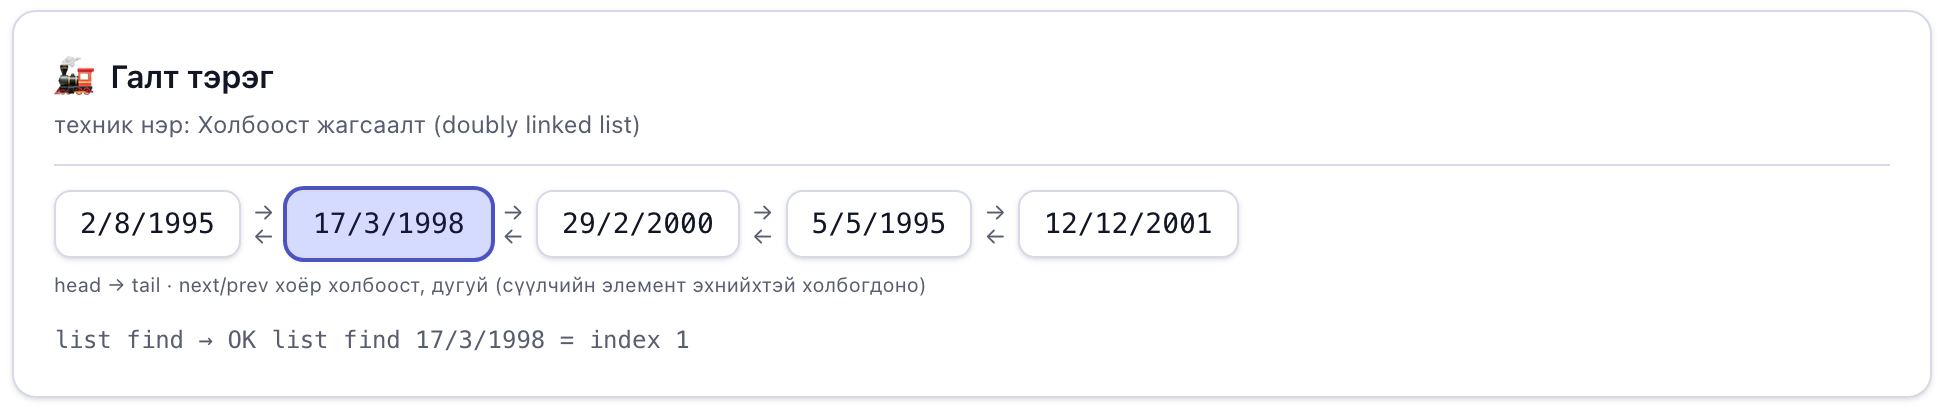
\includegraphics[width=0.95\textwidth,height=0.40\textheight,keepaspectratio]{ui_play_list.png}
\caption*{Зураг 2 -- Холбоост жагсаалт: 5 төрсөн өдрийг \code{add_tail}-аар дараалуулан оруулж, дараа нь \code{list find 17 3 1998}. Олдсон элемент (index 1) тодотгогдож, зангилаа бүрийн хооронд next/prev хоёр холбоос харагдана.}
\end{figure}

\begin{figure}[H]
\centering
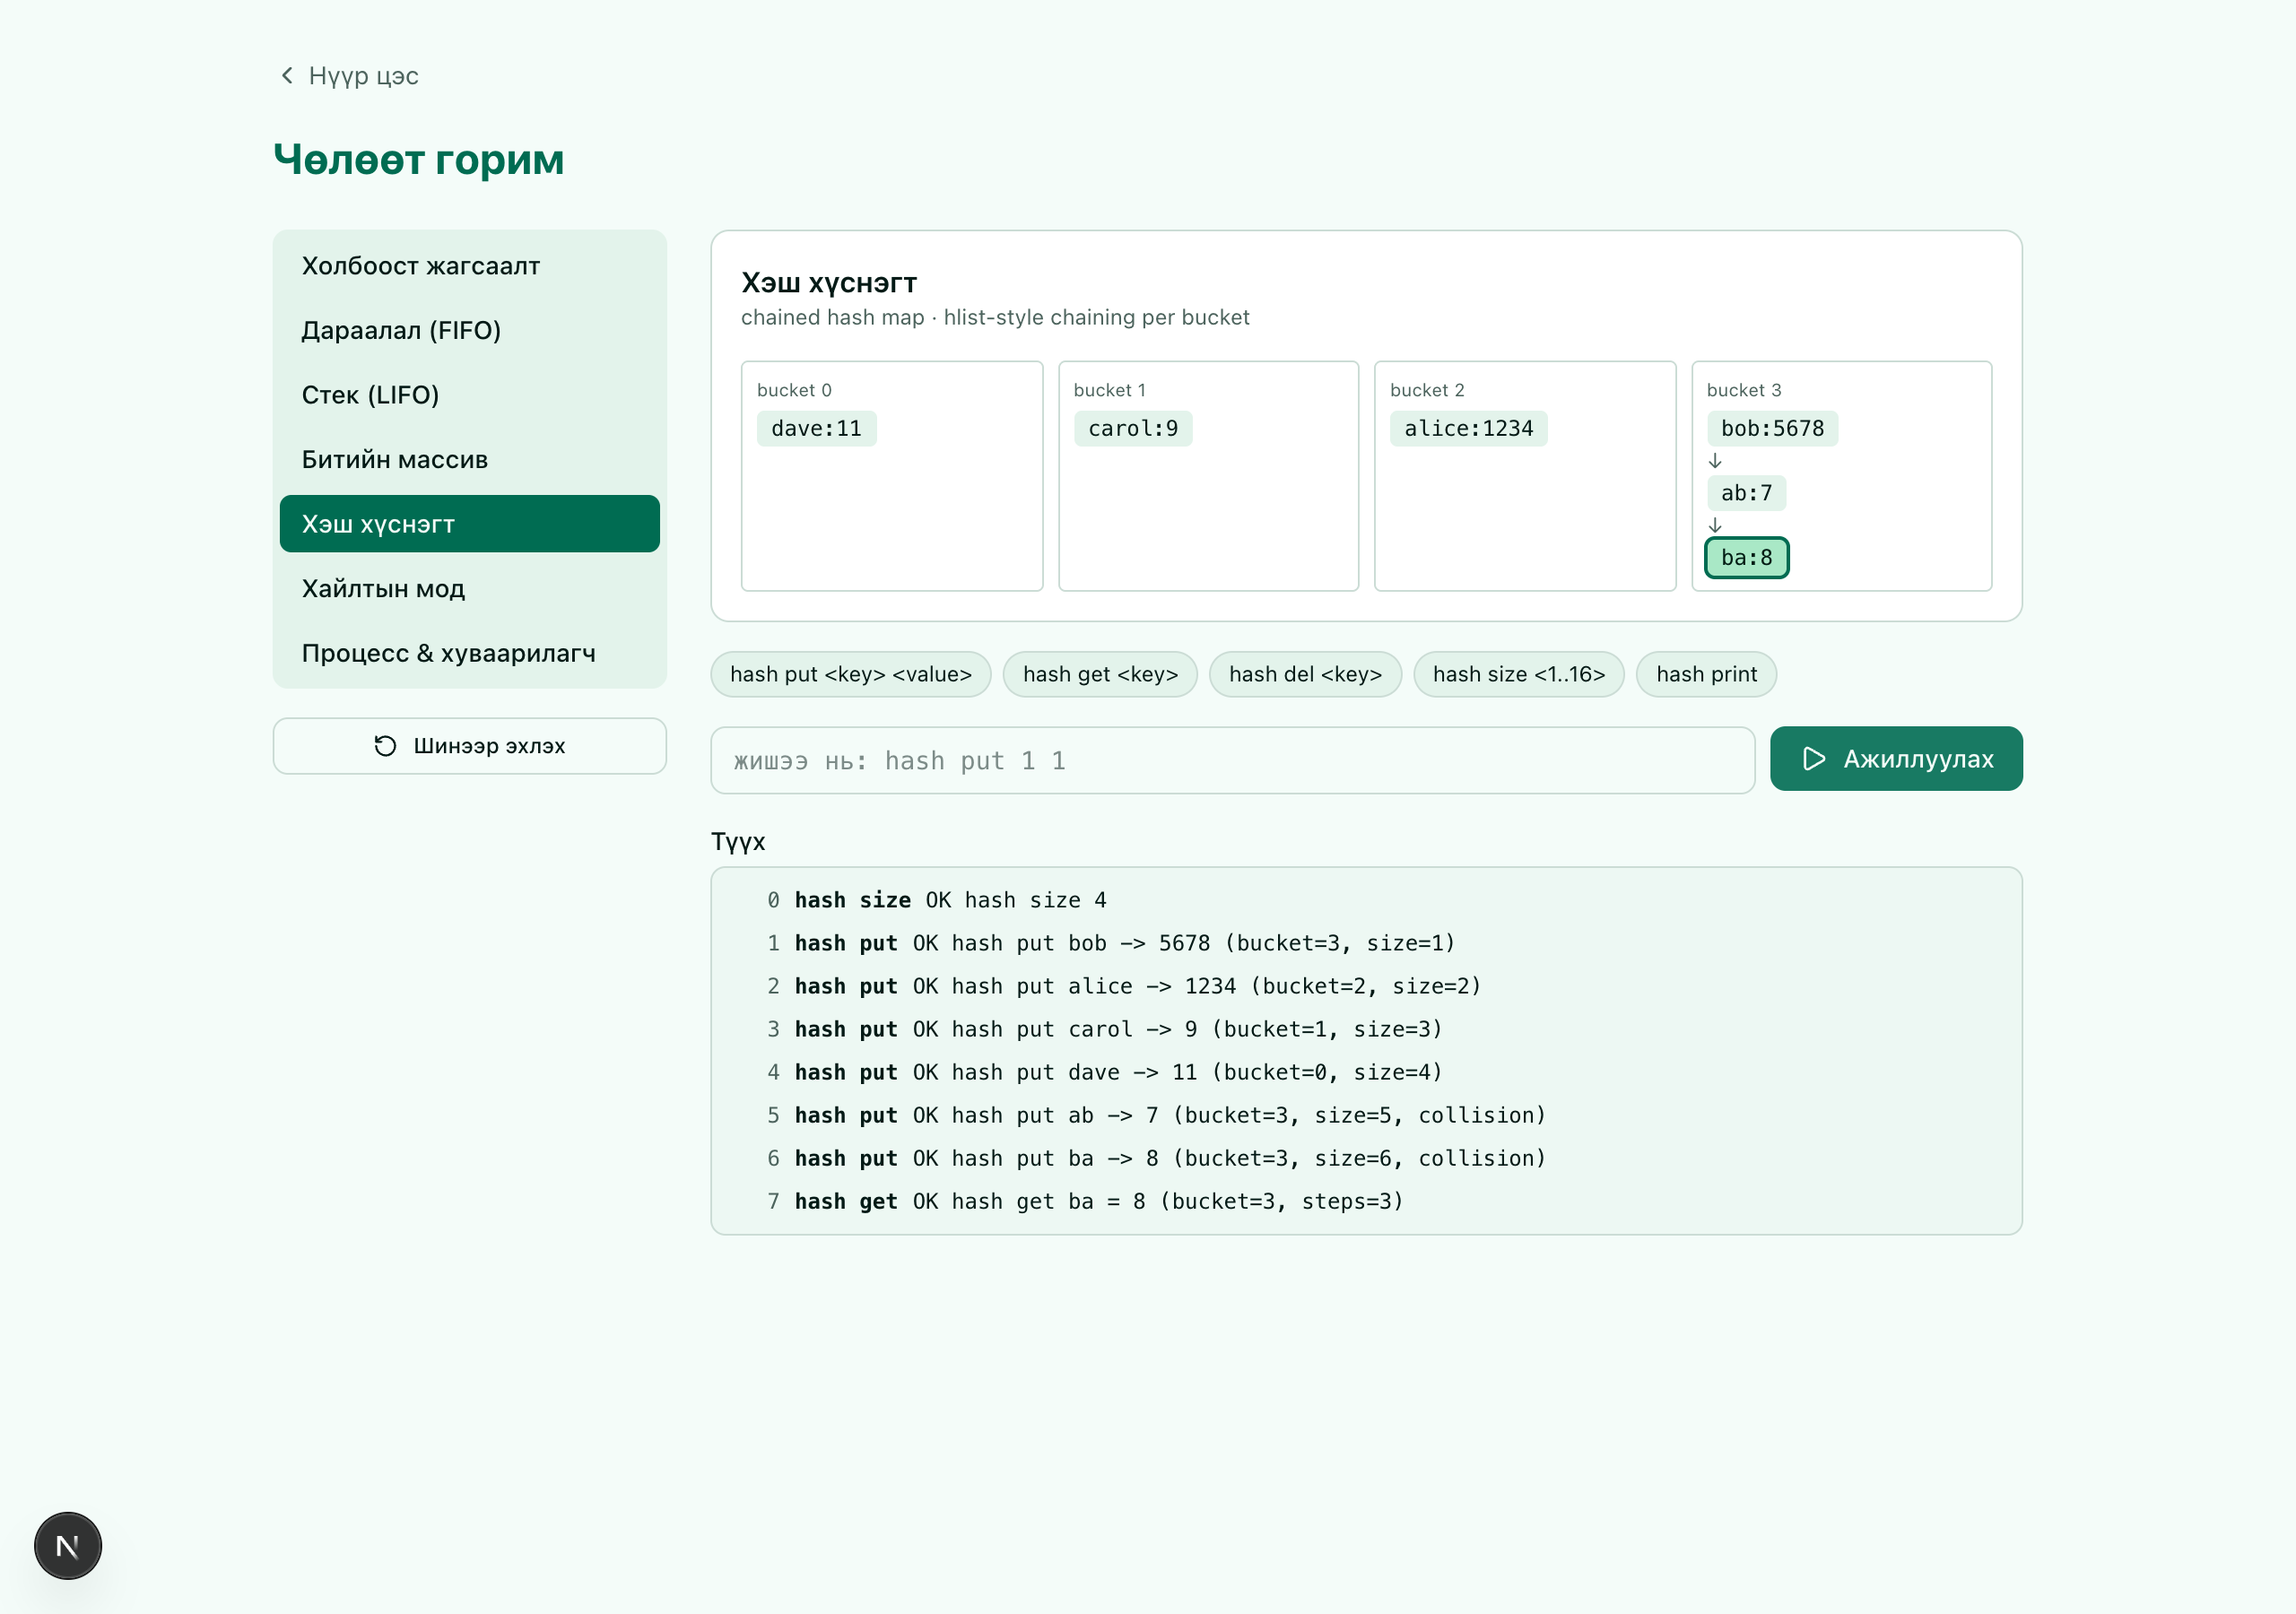
\includegraphics[width=0.95\textwidth,height=0.40\textheight,keepaspectratio]{ui_play_hash.png}
\caption*{Зураг 3 -- Хэш хүснэгт (4 bucket): \code{bob}, \code{ab}, \code{ba} нэг bucket-д унаж collision үүсэв; bucket 3 дотор chaining жагсаалт ба \code{hash get ba}-ийн steps=3 харагдана.}
\end{figure}

\begin{figure}[H]
\centering
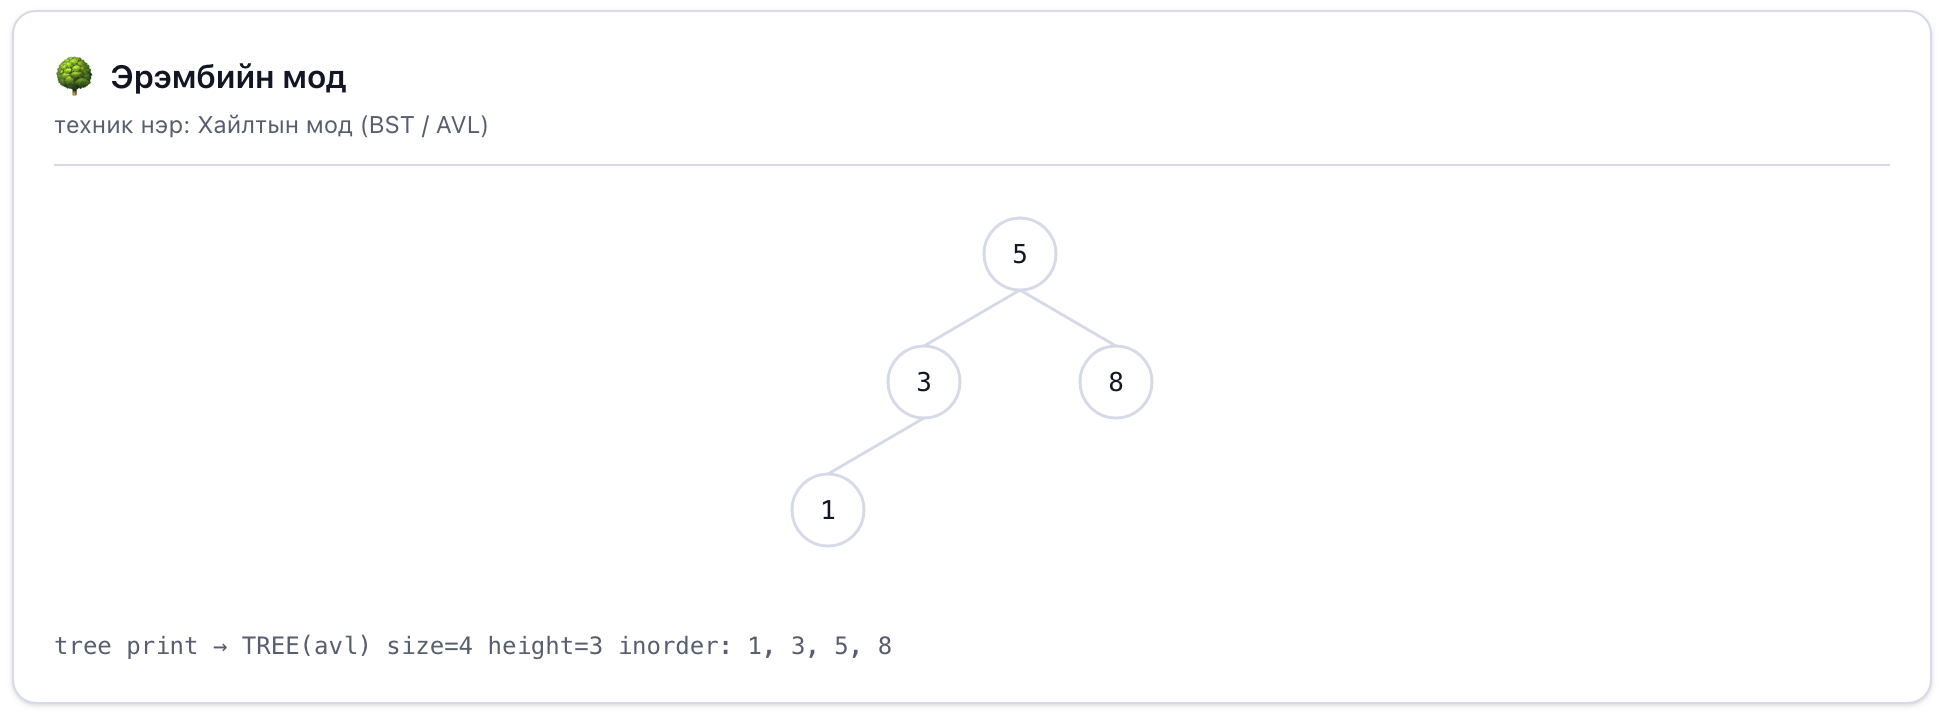
\includegraphics[width=0.95\textwidth,height=0.40\textheight,keepaspectratio]{ui_learn_tree.png}
\caption*{Зураг 4 -- AVL мод: 5, 3, 8, 1 оруулсны дараах граф; ирмэг (parent--child) ба inorder 1, 3, 5, 8. Энгийн BST-д ижил дараалал нэг шугам болдог бол AVL өндрийг 3-д барина.}
\end{figure}

\begin{figure}[H]
\centering
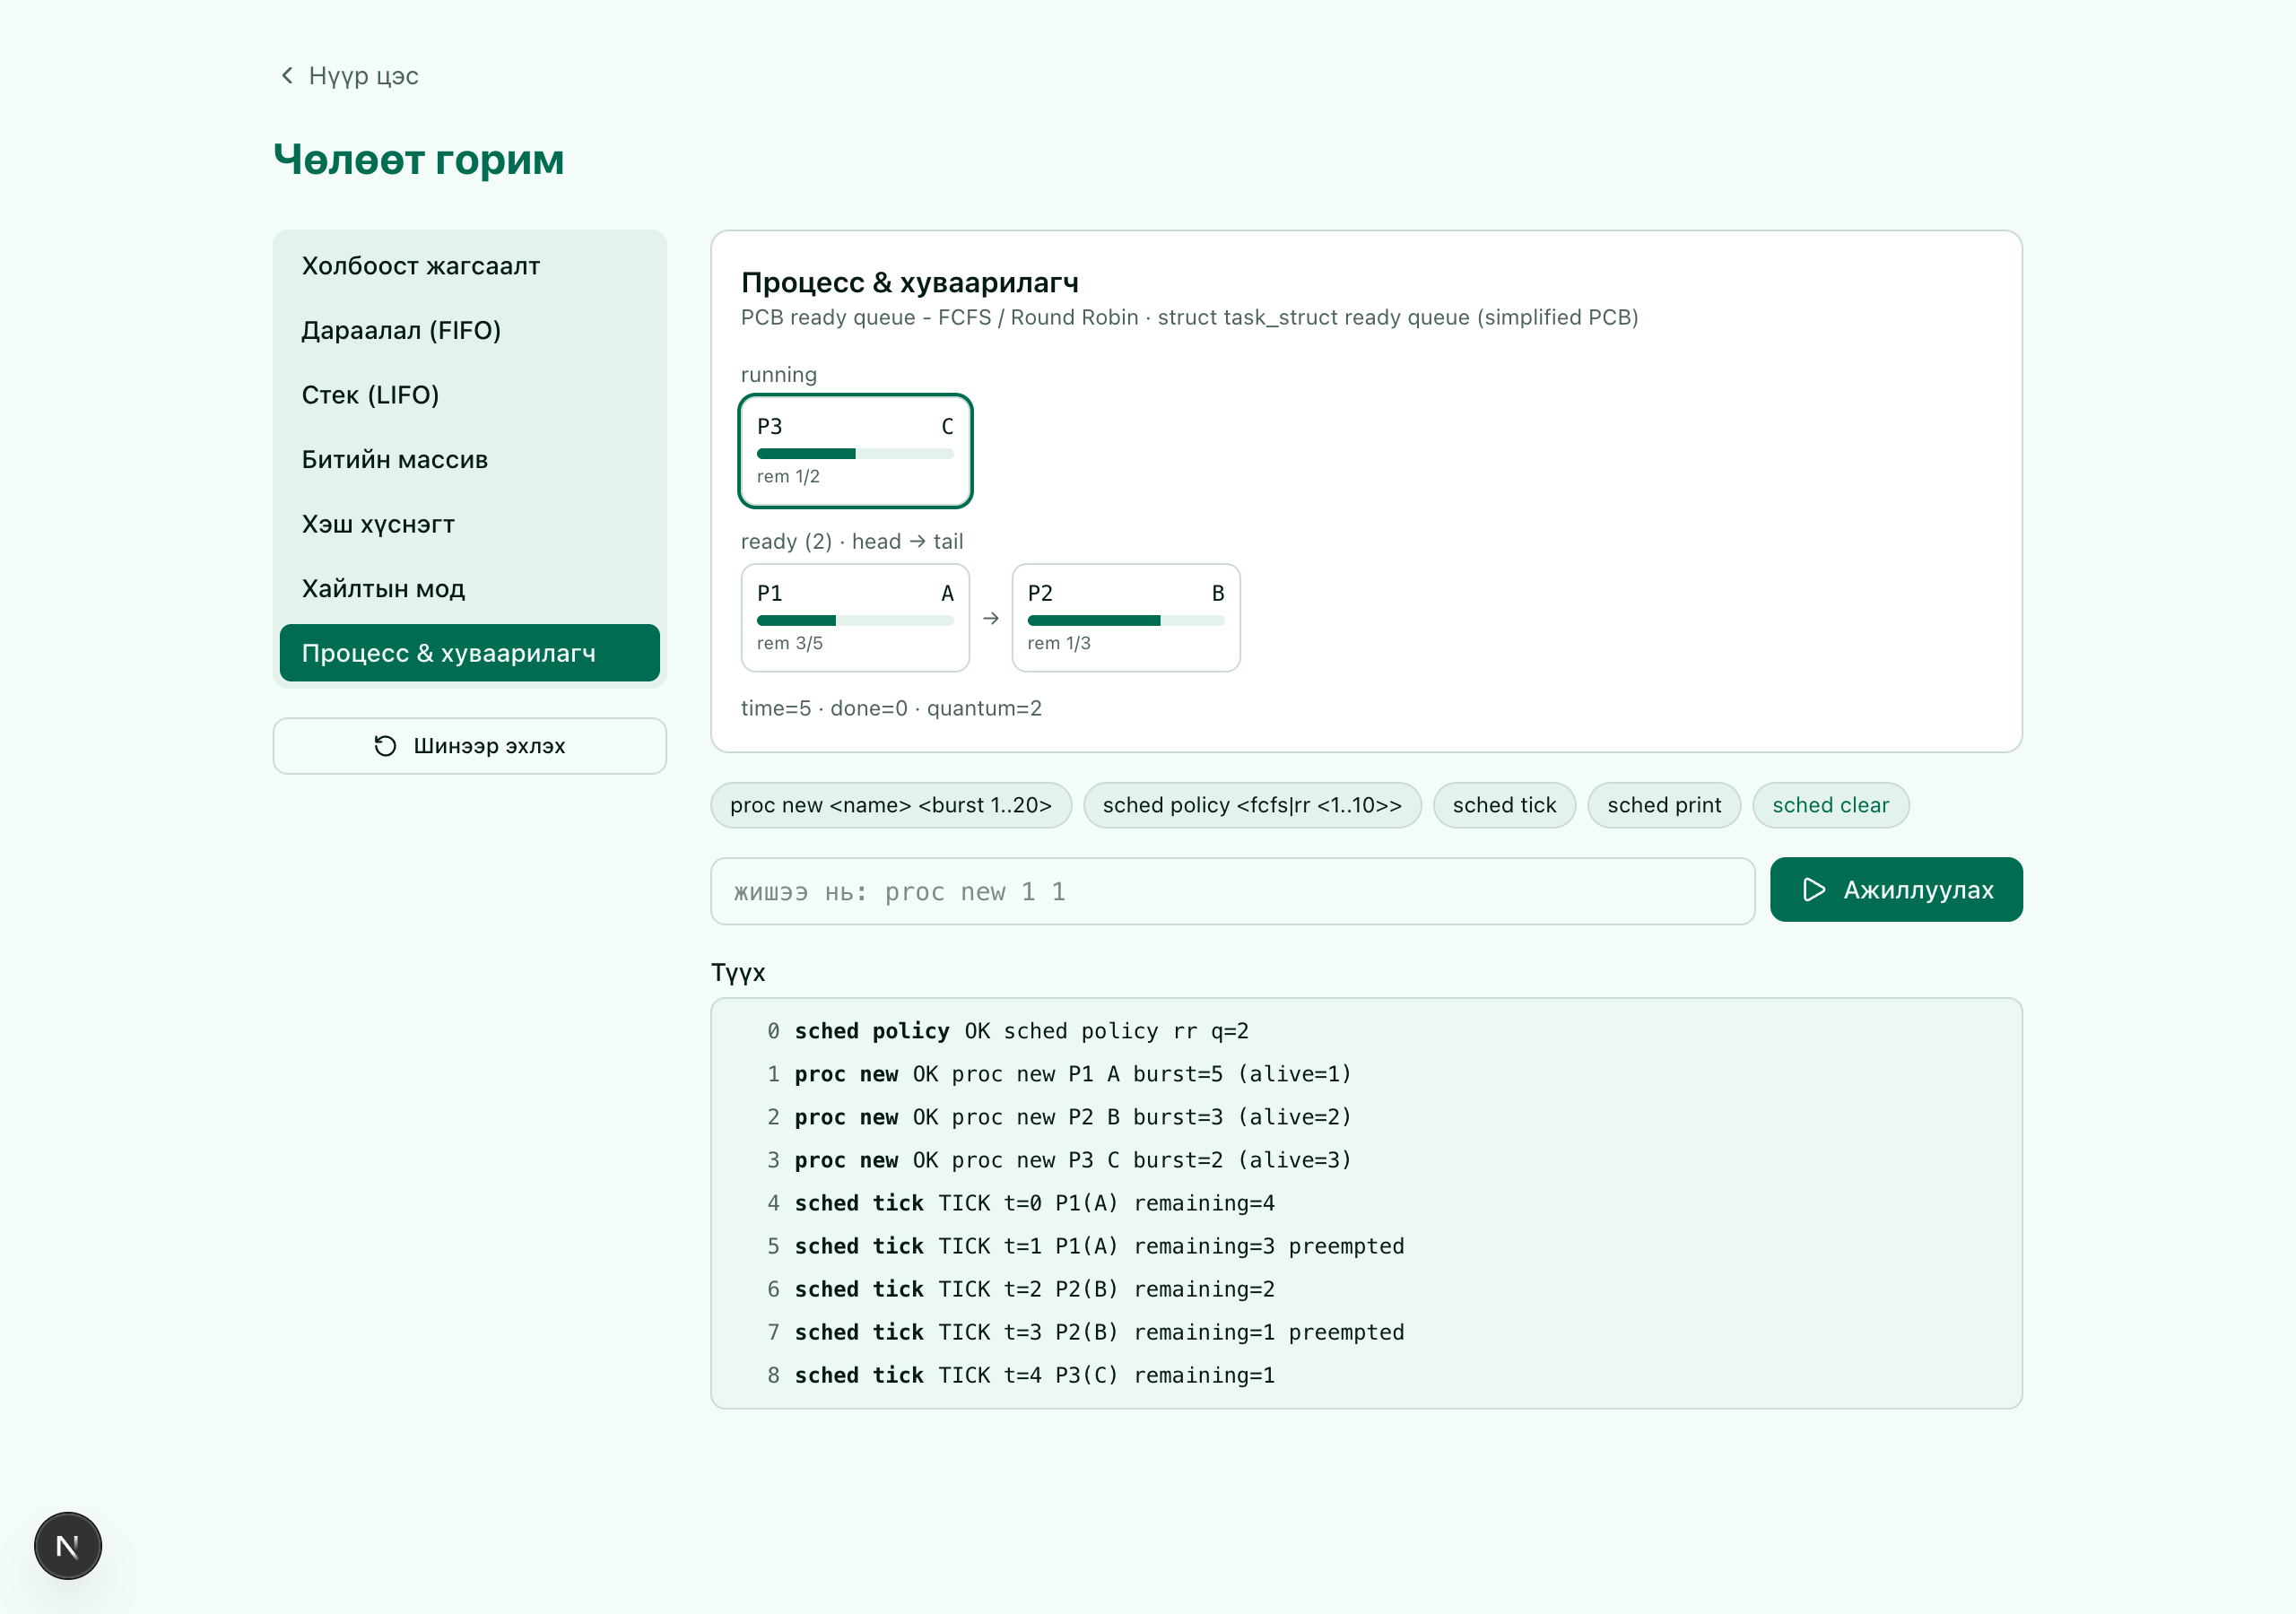
\includegraphics[width=0.95\textwidth,height=0.40\textheight,keepaspectratio]{ui_play_sched.png}
\caption*{Зураг 5 -- Round Robin (q=2): running P3, ready queue P1 $\rightarrow$ P2, процесс бүрийн progress bar (rem/burst), time=5, done=0. Ready queue нь \code{list_head} тул сум нь дараагийн PCB-г заана.}
\end{figure}

% ---------------------------------------------------------------------------
% 7. Туршилтын арга
% ---------------------------------------------------------------------------
\section*{7. Туршилтын арга}
\phantomsection\addcontentsline{toc}{section}{7. Туршилтын арга}

\textbf{Орчин:} Ubuntu 24.04, gcc 13, GNU make, Node.js 22 (веб апп, CI), Python 3.13 (тест скрипт). Kernel module-д Ubuntu 24.04, kernel 6.11.0-17-generic, linux-headers.

\textbf{Өгөгдөл ба хүлээгдэх үр дүн} (хүлээгдэх гаралт \code{tests/expected_*.out}-д хадгалагдсан):

{\fontsize{9.5}{12}\selectfont
\begin{longtable}{|L{0.16\textwidth}|L{0.40\textwidth}|L{0.37\textwidth}|}
\hline
\rowcolor{headbg}\textbf{Тест} & \textbf{Оролт / нөхцөл} & \textbf{Хүлээгдэх үр дүн} \\ \hline
\endfirsthead
\hline
\rowcolor{headbg}\textbf{Тест} & \textbf{Оролт / нөхцөл} & \textbf{Хүлээгдэх үр дүн} \\ \hline
\endhead
textbook & examples/textbook.txt -- сурах бичгийн 5 төрсөн өдөр, гүйлгэх, бүгдийг устгах & Оруулсан дарааллаар жагсаж, эцэст нь хоосон \\ \hline
all\_structures & queue, stack, bitmap, tree & FIFO/LIFO дараалал, bitmap 1000000000000001, inorder 20, 40, 50, 70 \\ \hline
errors & 31/4, 29/2/1900, сар 13, жил 1800, хоосноос pop, size 0/129, индекс $-1$/99, давхардсан утга & Мөр бүр ойлгомжтой ERR, програм унахгүй \\ \hline
search & Бүх бүтцэд хайлт, hash collision, BST 1--5, AVL 1--7 & index/position/steps, BST өндөр 5, AVL өндөр 3 \\ \hline
scheduler & RR q=2 ба FCFS: A=5, B=3, C=2; буруу нэр, ажил, бодлого & Гараар тооцсон хуваарьтай таарна (8-р хэсэг) \\ \hline
scheduler\_full & 9 процесс үүсгэх & 9 дэх нь татгалзагдана, нэг нь дууссаны дараа зөвшөөрөгдөнө \\ \hline
stress & 5000 × (queue/stack push+pop, hash put+del, proc new+tick) & ERR 0, ASan/UBSan мэдээлэлгүй \\ \hline
text == --json & tests/json\_check.py: 8 скриптийг текст горим ба \code{--json} горимоор зэрэг ажиллуулах & Мессеж бүр мөр мөрөөрөө ижил, state бүр 7 бүтцийг агуулна \\ \hline
fuzz & tests/fuzz\_json.py: 8 seed × 5000 санамсаргүй команд (буруу огноо, том индекс, 8-аас олон процесс, урт түлхүүр г.м.) & Текст ба \code{--json} горимын мессеж ижил \\ \hline
avl\_check & tests/avl\_check.py: 30 санамсаргүй гүйлт (50--400 insert/delete) & Inorder = эрэмбэлсэн олонлог, өндөр $\le 1.44\cdot\log_2(n+2)$ \\ \hline
kernel module & src/kernel/run\_module\_test.sh: start=25, start=15, start=0 & 24 ба 18 гишүүнтэй Collatz, start=0 үед $-EINVAL$ \\ \hline
\end{longtable}
\par}

Fuzz тест алдааг илрүүлж чадаж байгаа эсэхийг шалгахын тулд C-ийн AVL-ийн давхар эргүүлэлтийг зориуд устгаж туршсан. Ингэхэд seed 2 ба 4 нь модны өндрийн зөрүүг шууд илрүүлсэн тул тест үр дүнтэй болох нь батлагдсан.

% ---------------------------------------------------------------------------
% 8. Үр дүн
% ---------------------------------------------------------------------------
\section*{8. Үр дүн}
\phantomsection\addcontentsline{toc}{section}{8. Үр дүн}

{\fontsize{9.5}{12}\selectfont
\begin{longtable}{|L{0.55\textwidth}|L{0.40\textwidth}|}
\hline
\rowcolor{headbg}\textbf{Тест} & \textbf{Үр дүн} \\ \hline
\endfirsthead
\hline
\rowcolor{headbg}\textbf{Тест} & \textbf{Үр дүн} \\ \hline
\endhead
textbook, all\_structures, errors, hash\_resize, rb\_heap & \textcolor{passgreen}{\textbf{PASS ×5}} \\ \hline
search (хайлт, hash, BST/AVL) & \textcolor{passgreen}{\textbf{PASS}} \\ \hline
scheduler (RR, FCFS, алдаа), scheduler\_full (8 процесс) & \textcolor{passgreen}{\textbf{PASS ×2}} \\ \hline
stress (5000 × 8 команд) & \textcolor{passgreen}{\textbf{PASS, ERR 0, sanitizer мэдээлэлгүй}} \\ \hline
text == --json (8 скрипт) & \textcolor{passgreen}{\textbf{PASS ×8}} \\ \hline
fuzz text == json (8 seed × 5000 команд, тэгш seed-д AVL) & \textcolor{passgreen}{\textbf{PASS ×8 (seed бүрд ≈4\,700 гаралтын мөр)}} \\ \hline
avl\_check (30 гүйлт + эрэмбэлсэн 1..15) & \textcolor{passgreen}{\textbf{PASS ×32 (BST өндөр 15, AVL өндөр 4)}} \\ \hline
rb\_check (red-black 30 seed + min-heap 10 seed: өнгө, black-height, inorder/эс хазайх чанар) & \textcolor{passgreen}{\textbf{PASS ×40}} \\ \hline
Kernel module, баталгаажуулсан хувилбар (birthday, kfifo, bitmap) & \textcolor{passgreen}{\textbf{PASS: Ubuntu 24.04, kernel 6.11.0-17, insmod/rmmod (Зураг 1)}} \\ \hline
CI (GitHub Actions) & \textcolor{passgreen}{\textbf{PASS: C цөм (Ubuntu+macOS) ба Next.js веб апп build+тест}} \\ \hline
Kernel module-ийн шинэчлэгдсэн хэсэг (hashtable.h, rbtree.h, /proc/kds) & Жинхэнэ Linux дээр \code{run_module_test.sh}-ээр баталгаажуулна (CI Linux job build л хийнэ). Хүлээгдэх гаралтыг доор үзүүлэв. \\ \hline
\end{longtable}
\par}

\hthree{Сурах бичгийн жишээний бодит гаралт (examples/textbook.txt)}

\begin{codeblock}
OK list add_tail 2/8/1995 (size=1)
OK list add_tail 17/3/1998 (size=2)
OK list add_tail 29/2/2000 (size=3)
OK list add_tail 5/11/2001 (size=4)
OK list add_tail 30/12/2003 (size=5)
LIST size=5: 2/8/1995 -> 17/3/1998 -> 29/2/2000 -> 5/11/2001 -> 30/12/2003
OK list del 17/3/1998 (size=4)
LIST size=4: 2/8/1995 -> 29/2/2000 -> 5/11/2001 -> 30/12/2003
OK list del 2/8/1995 (size=3)   ...   OK list del 30/12/2003 (size=0)
LIST size=0: (empty)
\end{codeblock}

\hthree{Хайлт, хэш хүснэгт, мод (examples/search.txt, холбогдох мөрүүд)}

\begin{codeblock}
OK list find 17/3/1998 = index 1
OK list find 1/1/2001 = not found
OK queue find 20 = position 1
OK stack find 1 = position 2
OK hash put ab -> 7 (bucket=3, size=5, collision)
OK hash put ba -> 8 (bucket=3, size=6, collision)
HASH buckets=4 size=6 collisions=2: b0=[dave:11] b1=[carol:9] b2=[alice:1234] b3=[bob:5678 -> ab:7 -> ba:8]
OK hash get ba = 8 (bucket=3, steps=3)
OK hash get bob = 5678 (bucket=3, steps=1)
OK hash get zed = not found (bucket=3)
OK hash put bob = 0 (updated, bucket=3)
ERR hash: key and value must be 1..12 letters, digits or _
TREE size=5 height=5 inorder: 1, 2, 3, 4, 5
ERR tree: mode can only be changed when the tree is empty
TREE(avl) size=7 height=3 inorder: 1, 2, 3, 4, 5, 6, 7
TREE(avl) size=6 height=3 inorder: 1, 2, 3, 5, 6, 7
\end{codeblock}

\hthree{Scheduler: гараар тооцоо ба програмын гаралт}

Round Robin, квант 2; A=5, B=3, C=2 тик, бүгд t=0-д ирсэн. Тик t нь $[t, t+1)$ хугацааны завсар тул t=5 дээр дууссан процессын дуусах хугацаа 6 болно.

{\fontsize{9.5}{12}\selectfont
\begin{longtable}{|L{0.16\textwidth}|L{0.14\textwidth}|L{0.15\textwidth}|L{0.15\textwidth}|L{0.13\textwidth}|L{0.15\textwidth}|}
\hline
\rowcolor{headbg}\textbf{Процесс} & \textbf{Сүүлийн тик} & \textbf{Дуусах хугацаа} & \textbf{Нийт үргэлжилсэн} & \textbf{Ажил} & \textbf{Хүлээсэн} \\ \hline
\endfirsthead
\hline
\rowcolor{headbg}\textbf{Процесс} & \textbf{Сүүлийн тик} & \textbf{Дуусах хугацаа} & \textbf{Нийт үргэлжилсэн} & \textbf{Ажил} & \textbf{Хүлээсэн} \\ \hline
\endhead
C (P3) & 5 & 6 & 6 & 2 & 4 \\ \hline
B (P2) & 8 & 9 & 9 & 3 & 6 \\ \hline
A (P1) & 9 & 10 & 10 & 5 & 5 \\ \hline
\multicolumn{5}{|r|}{\textbf{Дундаж хүлээлт}} & \textbf{5.00} \\ \hline
\end{longtable}
\par}

Ижил ажлыг FCFS-ээр ажиллуулахад A 0, B 5, C 8 тик хүлээж, дундаж хүлээлт 4.33 болно. Round Robin богино процесст түргэн хариу өгдөг ч энэ жишээнд дундаж хүлээлт FCFS-ээс их гарсан нь квант ба шилжилтийн өртөг юм.

\begin{codeblock}
OK sched policy rr q=2
SCHED policy=rr(q=2) time=0 running=none ready=P1(A:5), P2(B:3), P3(C:2) done=0
TICK t=0 P1(A) remaining=4
TICK t=1 P1(A) remaining=3 preempted
TICK t=2 P2(B) remaining=2
TICK t=3 P2(B) remaining=1 preempted
TICK t=4 P3(C) remaining=1
TICK t=5 P3(C) remaining=0 finished
TICK t=6 P1(A) remaining=2
TICK t=7 P1(A) remaining=1 preempted
TICK t=8 P2(B) remaining=0 finished
TICK t=9 P1(A) remaining=0 finished
TICK t=10 idle
SCHED policy=rr(q=2) time=11 running=none ready=(empty) done=3
\end{codeblock}

\hthree{Буруу оролтын бодит гаралт (examples/errors.txt)}

\begin{codeblock}
ERR list: day out of range for month          (31/4/2000)
ERR list: day out of range for month          (29/2/1900 - өндөр жил биш)
ERR list: month must be 1..12
ERR list: year must be 1900..2100
ERR list: usage <op> <day> <month> <year>
ERR list: 1/1/2000 not found
ERR list: missing operation
ERR unknown structure 'frob'
ERR queue: underflow (empty)
ERR stack: underflow (empty)
ERR bitmap: size must be 1..128               (0 ба 129)
ERR bitmap: index 99 out of range 0..31
ERR tree: duplicate 5
ERR tree: 9 not found
\end{codeblock}

\hthree{Kernel module}

\begin{figure}[H]
\centering
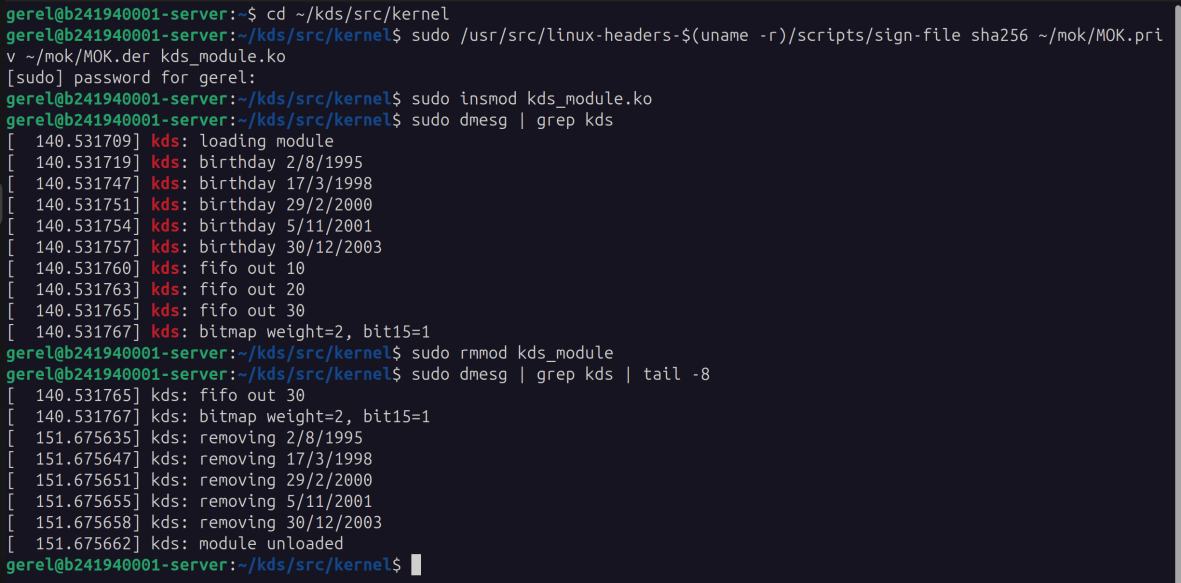
\includegraphics[width=0.90\textwidth,height=0.32\textheight,keepaspectratio]{dmesg_v1.png}
\caption*{Зураг 1 -- Kernel module-ийн өмнөх хувилбарын (birthday, kfifo, bitmap) бодит ачаалалт: Ubuntu 24.04, kernel 6.11.0-17-generic, MOK гарын үсэгтэй.}
\end{figure}

Part I/II нэмэгдсэн хувилбарын хүлээгдэх dmesg гаралт (\code{insmod kds_module.ko start=15}). Collatz гишүүдийг хэрэглэгчийн орчинд тооцоолж шалгасан: start=25 үед 24 гишүүн, start=15 үед 18 гишүүн.

\begin{codeblock}
kds: loading module (start=15)
kds: color red=255 blue=0 green=0
kds: color red=0 blue=255 green=0
kds: color red=0 blue=0 green=255
kds: color red=128 blue=64 green=32
kds: collatz 15
kds: collatz 46   23   70   35   106   53   160   80   40   20   10   5   16   8   4   2
kds: collatz 1
kds: collatz start=15 terms=18
kds: birthday 2/8/1995 ... 30/12/2003, fifo out 10 20 30, bitmap weight=2, bit15=1
(rmmod) kds: removing color ... / removing collatz 15 ... 1 / removing birthday ... / module unloaded
(insmod start=0) kds: start must be 1..1000000 (got 0)   -> insmod: Invalid parameters
\end{codeblock}

% ---------------------------------------------------------------------------
% 9. Хэлэлцүүлэг
% ---------------------------------------------------------------------------
\section*{9. Хэлэлцүүлэг}
\phantomsection\addcontentsline{toc}{section}{9. Хэлэлцүүлэг}

Бүх буруу оролт тодорхой мессеж өгч, програм нэг ч удаа унасангүй. ASan/UBSan санах ойн алдаа, leak мэдээлээгүй (Linux CI дээр; macOS 26 дээр \code{SAN=0} ажиллуулсан нь зөвхөн sanitizer шалгалтыг хасна). Веб апп нь бүтцийн логикийг дахин бичсэн хуулбар биш, зөвхөн C программаас ирсэн \code{--json} төлөвийг зурдаг тул «зураг бодит ажиллагаанаас зөрөх» асуудал угаасаа гарч ирэх боломжгүй; үүнийг 40\,000 санамсаргүй командад текст гаралт ба \code{--json} гаралтын мессеж яг таарч байгаагаар баталгаажуулсан (мөн энэ нь веб апп ямар JSON-г хүлээж авч байгааг шалгасан гэсэн үг). Эрэмбэлсэн оролтод BST-ийн өндөр n-тэй тэнцүү болж, AVL-ийнх $\lg n$ орчим байсан нь онолтой таарч байна. Хэш хүснэгтэд collision нэмэгдэх тусам хайлтын алхам өссөн нь мөн онолтой нийцнэ.

\Needspace{3\baselineskip}\textbf{Хязгаарлалт:}

\begin{enumerate}[leftmargin=22pt,itemsep=2pt,topsep=2pt]
  \item Kernel module-ийн өмнөх хувилбарыг нэг машин дээр (kernel 6.11.0-17) ачаалж туршсан. Өөр kernel хувилбарт дахин build хийх шаардлагатай. Secure Boot идэвхтэй үед гарын үсэггүй модуль ачаалагдахгүй тул MOK түлхүүрээр гарын үсэг зурсан.
  \item 1.9-д дурдсан red-black мод (\code{rbtree.h}) болон тусдаа singly жагсаалтыг хэрэгжүүлээгүй. Жагсаалт нь kernel-ийн list\_head шиг давхар холбоост дугуй, тэнцвэржсэн модыг AVL-аар загварчилсан.
  \item Хэш функц нь энгийн нийлбэр тул «ab», «ba» шиг үсгийн байр солигдсон түлхүүрүүд үргэлж collision үүсгэнэ. Bucket-ийн тоо auto resize-ээр 64 хүртэл ихэсдэг ч элементийн хязгаар 24-өөр бүдүүн дүрслэл болгож тоог хязгаарласан.
  \item Scheduler-т бүх процесс үүсгэсэн мөчдөө ирнэ гэж үзсэн. I/O хүлээлт ба тэргүүлэх эрэмбэ байхгүй.
  \item Веб апп зөвхөн дэлгэц дээр зурдаг, өөрөө логик агуулдаггүй тул интернэт/сервер шаардлагатай (хуучин нэг файлтай UI-гээс ялгаатай нь, тэр нь browser дотроо бүх логикыг давтдаг байсан). Веб аппыг локал ажиллуулахад \code{make}-аар \code{kds}-г урьдчилан build хийх шаардлагатай.
  \item Queue, stack ба амьд процессын тоо 8, hash-ийн элемент 24-өөр хязгаарлагдсан. Энэ нь дүрслэлд багтаах зорилготой.
\end{enumerate}

% ---------------------------------------------------------------------------
% 10. Дүгнэлт
% ---------------------------------------------------------------------------
\section*{10. Дүгнэлт}
\phantomsection\addcontentsline{toc}{section}{10. Дүгнэлт}

Сурах бичгийн 3-р бүлгийн «Kernel Data Structures» төслийн хоёр хэсэг (color жагсаалт, \code{start} параметртэй Collatz жагсаалт) болон 1.9-ийн бүтэц бүрийг хэрэгжүүлсэн: холбоост жагсаалт, дараалал, стек, BST ба тэнцвэржсэн мод, хэш хүснэгт, bitmap. Нэмэх, устгах, хайх үйлдлийн дараах төлөвийг CLI (текст) болон веб хуудас (граф) хоёуланд харуулж чадсан бөгөөд хоёулаа яг нэг C программаас ирсэн мэдээлэлд тулгуурладаг. Нүдээр харуулсан: энгийн мод эрэмбэлсэн оролтод нэг шугам болдог (өндөр 7) бол тэнцвэржсэн мод өндрөө 3 хэвээр хадгалдаг, хэш хүснэгтэд collision үүсэхэд хайлтын алхам нэмэгддэг. Зөв ажиллагааг 8 скрипт, stress тест, AVL, red-black ба min-heap-ийн инвариант шалгалт, текст==JSON харьцуулалт (40\,000 санамсаргүй команд), GitHub Actions дээрх автомат CI болон жинхэнэ Linux дээр ачаалсан kernel module-аар нотолсон. Нэмэлтээр «Processes» сэдвийн PCB ба ready queue ашиглан FCFS ба Round Robin-ийг хүлээлтийн хугацаагаар хэмжиж харьцуулсан.

% ---------------------------------------------------------------------------
% Ашигласан материал
% ---------------------------------------------------------------------------
\section*{Ашигласан материал}
\phantomsection\addcontentsline{toc}{section}{Ашигласан материал}

\begin{enumerate}[leftmargin=22pt,itemsep=2pt,topsep=2pt]
  \item A. Silberschatz, P. B. Galvin, G. Gagne. \textit{Operating System Concepts}, 10th ed. Wiley, 2018 -- Chapter 1 Introduction, 1.9 Kernel Data Structures (p. 36); 3-р бүлэг Processes ба Programming Projects.
  \item Linux kernel эх код ба баримт: \code{include/linux/list.h}, \code{include/linux/kfifo.h}, \code{include/linux/bitmap.h}, \code{include/linux/moduleparam.h}; Documentation/core-api/kernel-api.rst.
  \item The Linux Kernel Module Programming Guide (module\_param, insmod/rmmod).
  \item F.CSM302 «Бие даалт 1» удирдамж.
  \item AI хэрэгсэл: Claude (Anthropic) -- тайлангийн ноорог, C программын \code{--json} горим, веб апп (Next.js), CI/release тохиргоо, тест скрипт, баримт бичгийн засварт ашигласан. Бүх кодыг баг ажиллуулж, тестээр шалгасан.
\end{enumerate}

% ---------------------------------------------------------------------------
% Хавсралт A
% ---------------------------------------------------------------------------
\section*{Хавсралт A. Ажлын төлөвлөгөө ба гишүүдийн оролцоо}
\phantomsection\addcontentsline{toc}{section}{Хавсралт A. Ажлын төлөвлөгөө ба гишүүдийн оролцоо}

{\fontsize{9.5}{12}\selectfont
\begin{longtable}{|L{0.30\textwidth}|L{0.63\textwidth}|}
\hline
\rowcolor{headbg}\textbf{Талбар} & \textbf{Мэдээлэл} \\ \hline
\endhead
Хуваарилалтын код & V-1-4 \\ \hline
Төсөл & Kernel Data Structures \\ \hline
Repository & github.com/grl059/OS\_BD1 \\ \hline
Хэл / сан / орчин & C (gcc 13), TypeScript/React (Next.js), kernel C; Python 3, Node.js (тест, build); Ubuntu 24.04 \\ \hline
Үндсэн дүрслэл & Kernel structure graph -- веб апп (Next.js), 4 хуудастай (Нүүр, Чөлөөт горим, Хичээл, Тухай) \\ \hline
\end{longtable}
\par}

{\fontsize{9.5}{12}\selectfont
\begin{longtable}{|L{0.19\textwidth}|L{0.41\textwidth}|L{0.33\textwidth}|}
\hline
\rowcolor{headbg}\textbf{Гишүүн} & \textbf{Хариуцах ажил} & \textbf{Гаргасан файл / commit} \\ \hline
\endfirsthead
\hline
\rowcolor{headbg}\textbf{Гишүүн} & \textbf{Хариуцах ажил} & \textbf{Гаргасан файл / commit} \\ \hline
\endhead
Н. Ням-Од & Онолын судалгаа: сурах бичгийн Chapter 1, 1.9 Kernel Data Structures (p. 36) ба 3-р бүлгийн Programming Project, list\_head ба container\_of; тайлангийн 2--3-р хэсэг & 2026-10-27: UI граф, дэлгэцийн зураг, Report/Manual PDF, V-1-4 -- web/src/components/stage.tsx, docs/report\_src/*, docs/V-1-4\_*.pdf \\ \hline
А. Гэрэл & Repository удирдлага, веб апп (web/, Next.js) ба C программын \code{--json} горим, CI/release тохиргоо, C програм ба kernel module-ийг нэгтгэх, kernel module-ийг өөрийн Linux сервер дээр build хийж insmod/rmmod-оор турших; тайлангийн 4--6-р хэсэг & 2026-10-20…27: first commit, UI, Report zasav, Example, Code buten bolgov, JSON mode/web app/CI \\ \hline
А. Номин & Туршилтын өгөгдөл ба хүлээгдэх гаралт: 5 огнооны жагсаалт (textbook), бүх бүтцийн давхар тест (all\_structures), буруу/захын оролт (errors.txt: 31/4, 29/2/1900, сар 13, жил 1800, bitmap 0 ба 129, индекс $-$1 ба 99, давхардсан tree утга). Мөр бүрийн \code{ERR} мессежийг гараар уншиж \code{tests/run_tests.sh}-ийн жагсаалтад нэмсэн; тайлангийн 7-р хэсэг & examples/textbook.txt, examples/all\_structures.txt, examples/errors.txt, tests/expected\_errors.out, tests/run\_tests.sh \\ \hline
Э. Мягмаршагай & Процесс ба scheduler: A(5), B(3), C(2) процессийн RR (квант 2) ба FCFS хуваарийг хүснэгтээр гараар бодоод дуусах хугацаа 6/9/10, дундаж хүлээлт 5.00 ба 4.33-ыг \code{kds}-ийн гаралттай тулгасан; 8 процессийн \code{scheduler\_full}-д 9 дэх процесс татгалагдахыг шалгасан; тайлангийн 8-р хэсэг & examples/scheduler.txt, examples/scheduler\_full.txt, tests/expected\_scheduler.out, tests/expected\_scheduler\_full.out \\ \hline
О. Хүслэн & Manual (хэрэглэгчийн ба operational заавар) бичиж, хэсэг бүрийг дагаж өөр компьютер дээр \code{make}, \code{make test}, \code{make check}, \code{npm install}, \code{npm run dev}-ийг гүйцэтгэж, зааварт бичсэн хүлээгдсэн гаралттай таарч байгааг гараар тулгаж шалгасан & docs/latex/manual.tex, docs/report\_src/manual.html, docs/V-1-4\_Manual.pdf \\ \hline
Ч. Түмэншагай & Hash map ба AVL модны туршилт: «ab»/«ba» түлхүүрийн collision, bucket доторх хайлтын алхам, эрэмбэлсэн 1--7 оролтод BST өндөр 7 ба AVL өндөр 3-ыг гараар шалгасан; веб аппын хуудас бүрийн монгол тайлбар; тайлангийн 6, 9, 10-р хэсэг & examples/search.txt, tests/avl\_check.py, web/src/lib/levels.ts, web/src/app/about/page.tsx \\ \hline
\end{longtable}
\textbf{Тэмдэг:} Ажил тус бүрийг багийнхан хамтдаа хийж, бие биенийхээ гаралтыг шалгасан ч GitHub дээрх commit/push-ийг нэг гишүүн төвлөрүүлж хийдэг байсан тул \code{git log}-д гишүүн бүрийн нэр тус тусдаа гаргаагүй. Үүнийг \code{git shortlog}-ийн оронд дээрх файл, тестийн нэрээр баталгаажуулсан (жишээ нь \code{make test}-ийн 9 PASS мөр, \code{tests/expected\_*.out}-ын гаралт).
\par}

{\fontsize{9.5}{12}\selectfont
\begin{longtable}{|L{0.08\textwidth}|L{0.40\textwidth}|L{0.45\textwidth}|}
\hline
\rowcolor{headbg}\textbf{Тест} & \textbf{Оролт / нөхцөл} & \textbf{Хүлээгдсэн үр дүн} \\ \hline
\endhead
1 & examples/textbook.txt & 5 огноо дарааллаараа, устгасны дараа хоосон \\ \hline
2 & examples/search.txt & Хайлтын индекс, hash collision 2, BST өндөр 5, AVL өндөр 3 \\ \hline
3 & examples/scheduler.txt & RR дундаж хүлээлт 5.00, FCFS 4.33 \\ \hline
4 & examples/errors.txt & Мөр бүр ERR, програм унахгүй \\ \hline
5 & insmod kds\_module.ko start=15 & 4 color, 18 гишүүнтэй Collatz; start=0 $\rightarrow$ татгалзана \\ \hline
\end{longtable}
\par}

\end{document}
